\documentclass[10 pt, a4paper]{beamer}
\usetheme{metropolis}          
\usecolortheme{metropolis} 
\usepackage[utf8]{inputenc}
\usepackage{amsmath,amsfonts,amssymb}
\usepackage{dsfont}
\usepackage{graphicx}
\usepackage{caption}
\usepackage[french]{babel}
\usefonttheme[onlymath]{serif}

%partie 1 : pres des réseaux

%- def (cf rapport) + mise en forme matricielle 
%- dessins / exemples simples
%- LWE
%- BDD (et un peu SVP/CVP)
%- structure
%- PLWE et MPLWE (présentés avec Rot et Toep en forme matricielle)
%- ils sont q-ary + rang plein
%- Réduction Rosca 

%partie 2 : moi mdr

%- explication du but du stage
%- gamma BDD + heuristique gaussienne
%- volume (cas particulier rang plein qu'on garde dans la suite)
%- mes résultats
%- erreurs (trivial)
%- preuve heuristique gaussienne


% CITE KATARINA POUR LES IMAGES !

\title{Étude du problème MP-LWE}
\date{31 Août 2023}
\author{Sacha Ben-Arous}
\institute{ENS Paris-Saclay}
\begin{document}
  \maketitle
  
\begin{frame}{Plan}
\tableofcontents
\end{frame}  

\section{Introduction aux réseaux}

\subsection{Définition}
\begin{frame}{Définition}
\onslide<1->{Un \textbf{réseau euclidien} de $\mathbb{R}^m$ est l'ensemble des combinaisons à coefficients entiers de vecteurs linéairements indépendants $b_1, \dots, b_n$, que l'on note :
\[\mathcal{L}(b_1,\dots,b_n) := \left\{ \sum_{i=1}^n x_ib_i, x_i \in \mathbb{Z} \right\} \]}

\onslide<2->{Le réseau est alors de \textit{dimension} $n$, et la famille des $(b_i)_{1\leq i \leq n}$ est appelée \textbf{base} de ce réseau.}\\
\onslide<3->{~ \\ En notant $B:=[b_1,\dots,b_n]$ la matrice dont les colonnes sont formées par les $(b_i)_{1\leq i \leq n}$, on considérera de manière équivalente : \[\mathcal{L}(B) := \left\{ Bx, x \in \mathbb{Z}^n \right\} \]}
\end{frame}

\begin{frame}{Exemples}
Insérer des illustrations svp (si possible dimension 2 et 3 et q-ary et plusieurs bases pour un même réseau)
\end{frame}

\subsection{Learning With Errors}
\begin{frame}{Learning With Errors}
\textbf{Learning With Errors Problem :} \\ ~ \\
\onslide<1->{On fixe des entiers $n$ et $t$, un nombre premier $p$ et une distribution de bruit $\chi$. On tire un secret $s\hookleftarrow \mathcal{U}(\mathbb{Z}_p^n)$.  \\ ~ \\}

\onslide<2->{Le problème est le suivant : à partir de $t$ échantillons \[(a_i,b_i):=(a_i,\left<a_i,s\right> +e_i \text{ mod } p)\] où $a_i\hookleftarrow \mathcal{U}(\mathbb{Z}_p^n)$ et $e_i\hookleftarrow \chi$, on souhaite retrouver le secret $s$. \\ ~ \\}
\onslide<3->{\underline{Rq} : Sans bruit, le problème est facile à résoudre.}
\end{frame}

\begin{frame}{Lien avec les réseaux}
Cela revient à chercher le point le plus proche de $A\cdot s + e$ dans le réseau engendré par \\ ~ \\ $A' := 
 \left[\begin{array}{c|ccc}
a_1 &q&\cdots & 0\\
\vdots & \vdots &\ddots & \vdots\\
a_t & 0 & \cdots &q\\
\end{array}\right]
\in \mathbb{Z}^{t\times (n+t)}$
\\ ~ \\



\end{frame}

\begin{frame}{Difficulté de LWE}

\onslide<1->{La difficulté de la résolution algorithmique de ce problème est relié au facteur $\gamma = \frac{\lambda_1}{\|e\|}$, où $\lambda_1$ est la norme du plus court vecteur non nul du réseau engendré par $A'$. \\ ~ \\}

\onslide<2->{Plus $\gamma$ est petit, plus le problème est dur, et inversement. \\ ~ \\}

\onslide<3->{Pour $\gamma$ polynomial en $n$, ce problème est conjecturé exponentiellement dur à résoudre, même sur un ordinateur quantique.}

\end{frame}

\begin{frame}{Variantes structurées}
\onslide<1->{Si on utilise LWE tel quel pour construire un protocole, ce dernier aura une efficacité très moyenne, étant donné que les calculs mis en jeu sont des produits de grandes matrices aléatoires. \\ ~ \\}
\onslide<2->{Stehlé \textit{et al.} [SSTX09], résout ce problème en utilisant des réseaux structurés : les calculs matriciels correspondent alors à des produits de polynômes, calculables plus rapidement. C'est la variante P-LWE \\ ~ \\}

\end{frame}

\begin{frame}{Illustration}
Concrètement, cela consiste à représenter matriciellement le produit de polynômes, et donc à mettre des blocs structurés dans $A$
\begin{center}
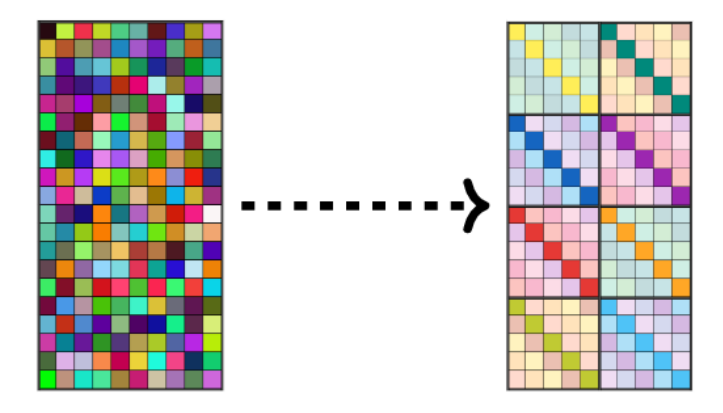
\includegraphics[scale=0.30]{plwe_struct.png}
\end{center}
\end{frame}

\begin{frame}{Variantes structurées}
\onslide<1->{Cependant, cette variante souffre encore d'un défaut : un nouveau paramètre $f \in \mathbb{Z}^n_p[X]$ est utilisé, et la complexité de P-LWE($f$) est directement liée au $f$ choisi. \\ ~ \\}
\onslide<2->{Roşca \textit{et al.} introduisent ainsi une nouvelle variante structurée, Middle-Product Learning With Errors, et prouve que des classes exponentiellement grandes de problèmes PLWE s'y réduisent, afin de se débarasser de la dépendance en $f$.}

\end{frame}

\begin{frame}{Représentation matricielle de la réduction}
Pour $f \in \mathbb{Z}^n_p[X]$ et $a \in \mathbb{Z}_p[X]$, on note $\text{Rot}_f(a) \in \mathbb{R}^{d\times m}$ la matrice dont la $i$-ème ligne est constituée des coefficients de $a\cdot x^{i-1}\text{ mod } f$.
\end{frame}

\end{document}













































